\documentclass[a4paper, 12pt]{tufte-book}

%\hypersetup{colorlinks}% uncomment this line if you prefer colored hyperlinks (e.g., for onscreen viewing)



%\renewcommand{\allcapsspacing}[1]{{\addfontfeature{LetterSpace=20.0}#1}}
%\renewcommand{\smallcapsspacing}[1]{{\addfontfeature{LetterSpace=5.0}#1}}
%\renewcommand{\textsc}[1]{\smallcapsspacing{\textsmallcaps{#1}}}
%
%% Will Robertson's fontspec.sty can be used to simplify font choices.
%\usepackage{fontspec,xltxtra,xunicode}
%\defaultfontfeatures{Mapping=tex-text}
%\setromanfont[Mapping=tex-text,Scale=0.95]{Palatino}%{Hoefler Text}
%%\setsansfont[Scale=MatchLowercase,Mapping=tex-text]{Gill Sans}
%\setmonofont[Scale=MatchLowercase]{Monaco}

%\usepackage[T1]{fontenc}
%\usepackage{inconsolata}
%\renewcommand*\ttdefault{lcmtt}

%%
% Book metadata
\title{Haskell as a\\ Platform for Game Development}

\author[Vic Smith, Laith Alissa, Jon Cave, Joseph Siddall]{Vic Smith, Laith Alissa, Jon Cave, \\Joseph Siddall}
\publisher{The Department of Computer Science\\University Of Warwick}

%%
% If they're installed, use Bergamo and Chantilly from www.fontsite.com.
% They're clones of Bembo and Gill Sans, respectively.
%\IfFileExists{bergamo.sty}{\usepackage[osf]{bergamo}}{}% Bembo
%\IfFileExists{chantill.sty}{\usepackage{chantill}}{}% Gill Sans

%\usepackage{microtype}

%%
% Just some sample text
\usepackage{lipsum}

%%
% For nicely typeset tabular material
\usepackage{booktabs}

%%
% For graphics / images
\usepackage{graphicx}
\setkeys{Gin}{width=\linewidth,totalheight=\textheight,keepaspectratio}
\graphicspath{{graphics/}}

% The fancyvrb package lets us customize the formatting of verbatim
% environments.  We use a slightly smaller font.
\usepackage{fancyvrb}
\fvset{fontsize=\normalsize}

\usepackage{amsmath}

% For ordinal number conversion
\usepackage{numname}

%%
% Prints argument within hanging parentheses (i.e., parentheses that take
% up no horizontal space).  Useful in tabular environments.
\newcommand{\hangp}[1]{\makebox[0pt][r]{(}#1\makebox[0pt][l]{)}}

%%
% Prints an asterisk that takes up no horizontal space.
% Useful in tabular environments.
\newcommand{\hangstar}{\makebox[0pt][l]{*}}

%%
% Prints a trailing space in a smart way.
\usepackage{xspace}

% Prints the month name (e.g., January) and the year (e.g., 2008)
\newcommand{\monthyear}{%
  \ifcase\month\or January\or February\or March\or April\or May\or June\or
  July\or August\or September\or October\or November\or
  December\fi\space\number\year
}

% Prints an epigraph and speaker in sans serif, all-caps type.
\newcommand{\openepigraph}[2]{%
  %\sffamily\fontsize{14}{16}\selectfont
  \begin{fullwidth}
  \sffamily\large
  \begin{doublespace}
  \noindent\allcaps{#1}\\% epigraph
  \noindent\allcaps{#2}% author
  \end{doublespace}
  \end{fullwidth}
}

\usepackage{changepage}

% Prints an epigraph for a chapter
\newcommand{\chapterepigraph}[2]{%
  %\sffamily\fontsize{14}{16}\selectfont
  %\begin{fullwidth}
  \vspace{1em}
  \begin{adjustwidth}{}{0.18\linewidth}
  \sffamily\small
  \noindent\raggedright\allcaps{#1}\\% epigraph
  \ -----\noindent\sc{ #2}% author
  \vspace{2em}
  \end{adjustwidth}
  %\end{fullwidth}
}

% Inserts a blank page
\newcommand{\blankpage}{\newpage\hbox{}\thispagestyle{empty}\newpage}

\usepackage{units}

% Typesets the font size, leading, and measure in the form of 10/12x26 pc.
\newcommand{\measure}[3]{#1/#2$\times$\unit[#3]{pc}}

% Generates the index
\usepackage{makeidx}
\makeindex

% Sort out part pages
\let\oldpart \part
\renewcommand{\part}[1]
{
	\begin{fullwidth}
		\oldpart[#1]{\normalfont#1}
	\end{fullwidth}
}

% Fix maketitle
\let\oldmaketitle \maketitle
\renewcommand{\maketitle}
{
	\newlength{\oldparindent}
	\newlength{\oldparskip}
	\setlength{\oldparindent}{\parindent}
	\setlength{\oldparskip}{\parskip}
	\setlength{\parindent}{0pt}
	\setlength{\parskip}{4pt}
	\oldmaketitle
	\setlength{\parindent}{\oldparindent}
	\setlength{\parskip}{\oldparskip}
}

%Configure the listings package
\usepackage{listings}

\lstdefinelanguage{Funk}
{
	alsoletter={:<>-=},
	morekeywords={interface, class, of, let, otherwise, case},
	morekeywords={extend, rename, as, redefine, data, events, depend, module},
	morekeywords={BEFORE, AFTER, AROUND, INTERCEPT, CONSTRUCTS, SENT, BY, SENDS, DURING},
	morekeywords={>>>, <<},
	morekeywords={new, defer, with},
	morekeywords={::, :=, ->, for},
	sensitive=true, 
	morecomment=[l]{//}, 
	morecomment=[l]{--}, 
	morecomment=[s]{/*}{*/}, 
	morestring=[d]{"},
	morestring=[b]{'},
}

% "define" Scala
\lstdefinelanguage{scala}{
  morekeywords={abstract,case,catch,class,def,%
    do,else,extends,false,final,finally,%
    for,if,implicit,import,match,mixin,%
    new,null,object,override,package,%
    private,protected,requires,return,sealed,%
    super,this,throw,trait,true,try,%
    type,val,var,while,with,yield},
  otherkeywords={=>,<-,<\%,<:,>:,\#,@},
  sensitive=true,
  morecomment=[l]{//},
  morecomment=[n]{/*}{*/},
  morestring=[b]",
  morestring=[b]',
  morestring=[b]"""
}

% "define" lolcode
\lstdefinelanguage{lolcode}{
  morekeywords={HAI,CAN, HAS, I, A, GIMMEH, IZ, BIGGER, THAN, YARLY, VISIBLE, NOWAI, KTHX, KTHXBYE},
  morecomment=[l]{BTW},
  morestring=[b]",
  morestring=[b]',
  morestring=[b]"""
}

\lstdefinelanguage[Objective]{C}[GNU99]{C}
  {morekeywords={@catch,@class,@encode,@end,@finally,@implementation,%
      @interface,@private,@protected,@protocol,@public,@selector,%
      @synchronized,@throw,@try,BOOL,Class,IMP,NO,Nil,SEL,YES,_cmd,%
      bycopy,byref,id,in,inout,nil,oneway,out,self,super,%
      % The next two lines are Objective-C 2 keywords.
      @dynamic,@package,@property,@synthesize,readwrite,readonly,%
      assign,retain,copy,nonatomic%
      },%
   moredirectives={import}%
  }%

\lstdefinelanguage[GNU99]{C}[99]{C}
  {morekeywords={asm,__asm__,__extension__,typeof,__typeof__}%
  }%

\lstdefinelanguage[99]{C}%
  {morekeywords={_Bool,_Complex,_Imaginary,auto,break,case,char,%
      const,continue,default,do,double,else,enum,extern,float,for,%
      goto,if,inline,int,long,register,restrict,return,short,signed,%
      sizeof,static,struct,switch,typedef,union,unsigned,void,volatile,%
      while},%
   sensitive,%
   morecomment=[s]{/*}{*/},%
   morecomment=[l]//,%
   morestring=[b]",%
   morestring=[b]',%
   moredelim=*[directive]\#,%
   moredirectives={define,elif,else,endif,error,if,ifdef,ifndef,line,%
      include,pragma,undef,warning}%
  }[keywords,comments,strings,directives]%

\lstset
{ 
	tabsize=4,
	showspaces=false,
	showstringspaces=false,
	upquote=true,
	breaklines=true,
	breakindent=4.5pt,
	basicstyle=\ttfamily,
	captionpos=t,         % sets the caption-position to top
	frame=none,
	aboveskip=1em,
	nolol=false,
	belowskip=1em,
	numberbychapter=true,
	escapechar=§,
}

% Customise listing captions
\usepackage{color}
\usepackage{xcolor}

\usepackage{caption}
\DeclareCaptionFont{gray}{\color{gray}}
\DeclareCaptionFormat{listing}
{
	\vspace{-1em}
	\parbox{\textwidth}
	{{\it#1#2}#3}
	\vspace{0.0em}
}
\captionsetup[lstlisting]{format=listing}
%%%%

% Use tocloft for finer control over lists and counters
\usepackage{tocloft}

\setcounter{tocdepth}{1}

%\renewcommand{\cftdotsep}{10}
\renewcommand{\cfttoctitlefont}{\huge\itshape}
\renewcommand{\cftloftitlefont}{\huge\itshape}
\renewcommand{\cftlottitlefont}{\huge\itshape}
\renewcommand{\cftchapfont}{\itshape\large}

\newcommand{\listofvlistingsname}{List of Listings}
\newlistof{vlisting}{vlist}{\listofvlistingsname}
\renewcommand{\cftvlisttitlefont}{\huge\itshape}

\newcommand{\setuplisting}[3]
{
	\refstepcounter{vlisting}
	\label{#1}
	\addcontentsline{vlist}{figure}{\thevlisting \hspace{15pt} #2 }
	\marginnote[2.5em]{Listing \thevlisting: #3}
}

\lstnewenvironment{listing}[4]
{%
	\lstset{#4}
	\setuplisting{#1}{#2}{#3}
}
{
}

% A punch card listing

\newcommand{\card}[1]{\fbox{#1}}

\newenvironment{punchcards}[3]
{%
	\vspace{0.5em}
	%
	\setuplisting{#1}{#2}{#3}
	%
	\noindent\rule{30em}{0.5pt}\\
	\vspace{0.3em}
	%
	\newlength{\oldparskip}
	\newlength{\oldparindent}
	%
	\setlength{\oldparskip}{\parskip}
	\setlength{\oldparindent}{\parindent}
	\setlength{\parskip}{0.4em}
	\setlength{\parindent}{0.7em}
}
{
	%\vspace{1em}
	\\ \noindent\rule{30em}{0.5pt}
	
	\vspace{1em}
	\setlength{\parskip}{\oldparskip}
	\setlength{\parindent}{\oldparindent}
}

% Macros

\newcommand{\Code}[1]{\lstinline{#1}}

\newcommand{\define}{\paragraph{Definition}}
\newcommand{\motivate}{\paragraph{Motivation}}

\newcommand{\arrownote}[1]
{
	\newlength{\lengthofarrow}
	\settowidth{\lengthofarrow}{$\leftarrow$}
	\marginnote{\hspace{-1.3em}$\leftarrow$ #1}
}
\usepackage{inlinebib}

\newcommand{\cneed}{\sidenote{CITATION NEEDED.}}

% Chapters in LOF
\usepackage{etoolbox}

\providebool{newchap}

%\let\oldcaption\caption
%\renewcommand{\caption}[2][\shortcaption]{%
%\def\shortcaption{#2}
%\ifbool{newchap}
%{%
%    \addcontentsline{lof}{chapter}{%
%        Chapter \thechapter: #1 \vspace{10pt}
%    }
%
%}{}
%    \global\boolfalse{newchap}
%    \oldcaption[#1]{#2}
%}

\makeatletter
\newcommand{\saved@chapter}{}
\let\saved@chapter\chapter
\newcommand{\chapterf}{%
  \@ifstar {\saved@chapter*}{\@dblarg\my@chapter}%
}
\newcommand*{\my@chapter}[2][]{%
  \saved@chapter[#1]{#2}%
  %\global\setbool{newchap}{true}
  \addcontentsline{lof}{chapter}{%
        #1 \vspace{10pt}
    }

}
\makeatother

\newcommand{\containsfigures}[1]
{\addcontentsline{lof}{chapter}{#1 \vspace{10pt}}
}

\newcommand{\containslistings}[1]
{\addcontentsline{vlist}{chapter}{#1 \vspace{10pt}}
}

\usepackage{amsthm}

\theoremstyle{plain} %default 
\newtheorem*{thm}{Theorem}
\newtheorem*{lem}{Lemma} 
\newtheorem*{prop}{Proposition} 
\newtheorem*{cor}{Corollary} 

\theoremstyle{definition} 
\newtheorem{defn}{Definition}
\newtheorem*{conj}{Conjecture}
\newtheorem*{exmp}{Example}
\newtheorem*{nota}{Notation}

\theoremstyle{remark} 
\newtheorem*{rem}{Remark} 
\newtheorem*{note}{Note} 
\newtheorem{case}{Case}

% Formal semantics commands
\newlength{\lengthofharpoon}
\settowidth{\lengthofharpoon}{$\leftharpoonup$}
\newcommand{\update}{\scalebox{0.95}{\,\raisebox{1pt}{$\leftharpoonup$}\hspace{-\lengthofharpoon}\raisebox{-1pt}{$\leftharpoondown$}}\,}
\newcommand{\tupdate}{\scalebox{0.95}{\,\raisebox{2pt}{$\leftharpoonup$}\hspace{-\lengthofharpoon}\raisebox{-2pt}{$\leftharpoondown$}}\hspace{-\lengthofharpoon}-}

\newcommand{\sig}{\varsigma}
\newcommand{\llp}{\llparenthesis}
\newcommand{\rrp}{\rrparenthesis}

\usepackage{stmaryrd}
\setcounter{secnumdepth}{2}

\begin{document}

% Front matter
\frontmatter

%% r.1 blank page
%\blankpage
%
%% v.2 epigraphs
%\newpage\thispagestyle{empty}
%\openepigraph{%
%The public is more familiar with bad design than good design.
%It is, in effect, conditioned to prefer bad design, 
%because that is what it lives with. 
%The new becomes threatening, the old reassuring.
%}{Paul Rand%, {\itshape Design, Form, and Chaos}
%}
%\vfill
%\openepigraph{%
%A designer knows that he has achieved perfection 
%not when there is nothing left to add, 
%but when there is nothing left to take away.
%}{Antoine de Saint-Exup\'{e}ry}
%\vfill
%\openepigraph{%
%The designer of a new system must not only be the implementor and the first 
%large-scale user; the designer should also write the first user manual\ldots 
%If I had not participated fully in all these activities, 
%literally hundreds of improvements would never have been made, 
%because I would never have thought of them or perceived 
%why they were important.
%}{Donald E. Knuth}


% r.3 full title page
\maketitle

%\addcontentsline{toc}{chapter}{Front Matter }

% v.4 copyright page
\newpage
\begin{fullwidth}
%    \addcontentsline{toc}{chapter}{Abstract and Bibliographic Information}%
	{\large {\it Authors\ \ } Vic Smith, Laith Alissa, Jon Cave, Joseph Siddall
	
	\vspace{1em}\noindent{\it Supervisor\ \ } Sara Kalvala
	
	\vspace{1em}\noindent{\it Client\ \ } Matthew Leeke
	
	\vspace{1em}\noindent{\it Abstract\ \ } A full multiplayer strategy game --- designed to be competitive in the current independent game market --- was developed and implemented exclusively using the Haskell language, with the goal of evaluating the efficacy of Haskell for development of this nature. Haskell was shown to be quite effective in this space, despite the pure functional nature of the language and the comparative lack of library support in the domain of games. Full details of the strengths and challenges of this approach are reported on herein, and a set of best practices for the use of Haskell in games development are suggested.
	
	\vspace{1em}\noindent{\it Keywords\ \ } Functional Programming, Haskell, Game Development, Graphical User Interface, Networking
	
	}
	
	~\vfill
	\thispagestyle{empty}
	\setlength{\parindent}{0pt}
	\setlength{\parskip}{\baselineskip}
	Copyright \copyright\ \the\year\ \plainauthor
	
	\par\smallcaps{Published by \newlinetospace{\thanklesspublisher}}
	
	%\par\smallcaps{Typesetting: tufte-latex.googlecode.com}
	
	\par\textit{First printing, \monthyear}

	\newpage

\end{fullwidth}

% Dedication
%~\vfill
%\begin{doublespace}
%\noindent\fontsize{18}{22}\selectfont\itshape
%\nohyphenation
%Dedicated to the Haskell Community, upon whose shoulders rest this and many other projects.
%\end{doublespace}
%\vfill
%\vfill


\begin{fullwidth}

\cleardoublepage

% Contents
%\addcontentsline{toc}{chapter}{Detailed Contents, Lists of Figures, Tables, and Listings}
\tableofcontents

\cleardoublepage
\phantomsection \label{listoffig}
%\addcontentsline{toc}{section}{List of Figures}
\listoffigures

\cleardoublepage
\phantomsection \label{listoflis}
%\addcontentsline{toc}{section}{List of Tables}
\listoftables

\cleardoublepage
\phantomsection \label{listoflis}
%\addcontentsline{toc}{section}{List of Listings}
\listofvlisting

\end{fullwidth}


%%
% Start the main matter (normal chapters)
% r.9 introduction

% \chapter{Foreword}

\newthought{Lorum ipsum} set dolor amet. \lipsum[2]

\mainmatter

\chapter[Beginnings: On Games and Functional Programming]{Beginnings: On Games and Functional Programming}
\label{ch:beginnings}
\containsfigures{Beginnings}
\containslistings{Beginnings}
\containstables{Beginnings}

\chapterepigraph{Advances in technology won't be as significant as they have been in the past, most games won't be materially improved by simulating every drop of water in the pond you are wading through. More resources can be profitably spent to make the creation process easier.}{John Carmack}

\chapter[Motivation]{Motivation}
\label{ch:motivation}

\chapterepigraph{If you aren't sure which way to do something, then do it both ways and see which works better.}{John Carmack}

\newthought{Functional programming} has a long history, with its roots in the $\lambda$-calculus of Alonzo Church.\citefix[-1.5em]{church1932} One of the first functional programming languages was Lisp, invented by John McCarthy in the 1958; and Lisp is still used today, over 50 years later.\citepage{reilly2003}{pages 156--157} Various languages have refined and extended the paradigm over the years --- probably the most notable as of now being Haskell, Scala, OCaml, F\#, and Erlang.

Despite the amount of time such languages have been available, use in industry has typically been far less than that of languages such as C, C++, and Java.\citepage[-2em]{odersky2010programming}{page 11} That being said, in recent years there has been increasing use of functional techniques and languages in certain areas. Erlang was designed for the development of highly fault tolerant telecommunication systems.\cite[-1em]{armstrong2007history} OCaml is used in the financial sector to create trading algorithms.\citefix[1em]{minsky2011ocaml} Scala is increasingly popular, helped 

One of the often cited reasons against the use of functional programming in some domains is that of performance. This is due in part to mutable data structures generally being easier to represent on machine hardware; and it therefore being harder for functional compilers to convert the code into an efficient representation.\citefix{paulson1996ml} However, it is not a given that any program would run slower if written in a functional language: in some cases lazy-evaluation or compiler optimisations made possible by immutability can mean a program runs faster, plus advanced compiler techniques such as array fusion can lead to programs nearing the efficiency of hand-crafted C. And with modern machines getting ever faster, the domain of problems that require high levels of efficiency is getting smaller.

Performance problems alone cannot account for the fringe position of functional programming. The efficacy and advantages of the functional approach to programming and problem solving have been stated many times over a considerable number of years,\citefix{hughes1989functional} yet it is still rare for mainstream projects to make any use of functional languages or tools.

Instead of researching and discussing the theoretical advantages of the functional paradigm, this project instead will attempt to demonstrate the value of functional programming by utilising it in a problem domain that should pose a significant  challenge, that is not normally considered a `good' domain for FP. 

\section{Why a Game?}

Game programming brings together a diverse range of computing areas. A game involves human interaction in real time, detailed graphics and animation, artificial intelligence / planning, networking, and various other dynamic elements. A game is also 

\section{Why Haskell?}
\section{Initial Design Work and Specification}

% The early conception of the project, leading up to the start of the prototypes.

Lorum ipsum sit dolor amet.\citefix{church1932}  \lipsum[2-4]
\chapter[Research and Development: Games in Space and Time]{Research and Development: Games in Space and Time}
\label{ch:rd}
%\containsfigures{Research and Development: Games in Space and Time}
%\containslistings{Research and Development: Games in Space and Time}
%\containstables{Research and Development: Games in Space and Time}

\chapterepigraph{A game is a series of interesting choices.}{Sid Meier}

\newthought{Brief intro} for this section. \lipsum[4]

\lipsum[4]

\clearpage\section{Pilot Projects: Conway's Game of Life, SpaceTime, and Moon Survival}

% Descriptions of pilot projects.

Lorum ipsum sit dolor amet.\citefix{church1932}  \lipsum[2-4]
\clearpage\section{Literature Review: Functional Programming for Games}
\label{sec:fp_review}

\label{cf:code_organisation} % Reference from architecture section on OO vs FP code structure

% Literature review of existing work
% What this review is
% Less about games, more about Haskell as a real world language ==> more literature
% Discuss paper, critique, explain relevance

This section will discuss the suitability of the functional approach, the use
of Haskell in particular, in the real world. It will look at past projects and
research into the use of functional programming languages in industry in an
attempt to discover how functional programming helped or hindered development.
% More intro

John Hughes' paper ``Why functional programming matters'' aims to demonstrate how
``vitally important'' functional programming is to the real world by exploring and
demonstrating its advantages.\cite{hughes1989whyfp} Hughes argues that modularity
is the key to designing and implementing successful programs for three main reasons.
Firstly, small modules are much easier to code quickly because the requirements for
a small component are much easier to reason about, design, and implement. Second,
the more generic modules that are constructed can be reused. This leads to faster
development during subsequent projects. Thirdly, the independence of modules allows
them to developed and tested separately, helping to parallelise the work that needs
to be done and reducing the amount of time required for debugging. These advantages
of modular design combine to bring great improvements to productivity. These benefits
of modularisation are also espoused by Parnas who agrees that modular programming
shortens development time, improves comprehensibility of the resulting programs,
and increases flexibility --- it is possible to make large changes to one module
without affecting any of the others.\cite{parnas1972modular}

However, the ability of the programmer to modularise their code is reliant on the
ways in which they can glue the solutions of subproblems together. This glue must
often be provided by the programming language itself. Hughes argues that functional
programming provides two very important kinds of glue: higher order functions
and lazy evaluation. These two aspects of functional programming are very powerful
and allow greatly improved modularisation.

\functions(reduce)
General higher order functions, such as "map" and "reduce"\sidenote{The \scalenote{"reduce"} function is called \scalenote{"foldl"} in Haskell}, can be used as glue for
simpler, specialised functions to make more complex ones. Higher order functions
are great examples of code reuse as they can be used to create many other functions
with minimal effort. Hughes gives examples of operations over lists and trees, such
as summing up the elements of a list, whose implementation is greatly simplified
by the use of higher order functions. Lazy evaluation, on the other hand, allows
whole programs to be glued together. When composing two programs it might be
infeasible to store the entirety of the output of the first function in memory to
pass on to the second. Lazy evaluation is a solution to this problem. The output
function is only started when the input to the second function is required, and
only runs for long enough to provide the required amount of input. If the consuming
function terminates early then the producer can also quit. This even allows the
producer to create an infinite amount of output. This allows modularisation by
constructing a generator that outputs a large set of potential answers and a
separate selector that chooses the correct one.

Hughes finishes with an example from the field of artificial intelligence, a
field of computer science that is very relevant to game development. He shows
how the alpha-beta pruning algorithm can be constructed relatively simply using
modularisation through higher order functions and lazy evaluation. The algorithm
works by generating the entire set of possible game states that are reachable
from the current position. This list can then be lazily evaluated to find the
optimal move, but without actually constructing the entire, possibly infinite,
game tree. Higher order functions are used throughout to build up complex
functions from simpler ones. Hughes also shows that due to the modularisation
of the example it is much easier to understand and make modifications to the
program.

This paper is a great example of the power of that is available from the functional
approach. Giving real examples Hughes is able to make a strong case for the
effectiveness of modularisation through laziness and higher order functions.
The demonstration of a highly modular version of the alpha-beta pruning algorithm,
in particular, is of great interest due to its applicability to game development.
The conclusion that the functional approach leads to more general, reusable
modules is supported by John Backus' ACM Turing award lecture from 1977. Backus
gives the example of a program to calculate the inner product and finds that
``the functional version is nonrepetitive, \ldots is more hierarchically constructed,
is completely general, and creates `housekeeping' operations by composing high-level
housekeeping operators.''\cite{backus1978liberate}

In his 1987 paper ``No Silver Bullet'', Brooks identified four difficulties that
are inherent in the nature of software development: complexity, conformity,
changeability, and invisibility.\cite{brooks1987bullet} Brooks believes that
these four essential difficulties make it very unlikely that there will be a
``single development, in either technology or in management technique,
that by itself promises even one order-of-magnitude improvement in productivity,
in reliability, in simplicity.'' However, Moseley and Marks argue that complexity
is the only significant problem; that ``complexity is \emph{the} root cause of the
vast majority of problems with software today.''\cite{moseley2006tarpit} Other
problems can either be classified as complexity, or derive from unmanageable
complexity. They argue that simplicity is vital to successful software development,
and that functional programming can help to deliver this simplicity.

Moseley and Marks indentify several causes of complexity in real software systems.
The first cause is mutable state. Brooks also mentions the problem of state,
saying that from ``the difficulty of enumerating, much less understanding, all
the possible states of the program, \ldots comes the unreliability''.\cite{brooks1987bullet}
State hinders understanding of software through testing and reasoning about the code.
This is because testing a program in one state does not guarantee anything about
how the program will behave when in a different state. The vast number of different
possible states also makes it infeasible to understand them all. The functional
solution to the complexity of state is to discard state and side effects.
Programming with a pure functional language, such as Haskell, creates referentially
transparent programs. Referential transparency means that given the same set of
arguments a function will \emph{always} return the same result. Removing state
and side effects eases understanding of programs because they are easier to
reason about and test: ``avoiding side effects has serendipitous effects on testing.''\cite{smallbone2011}

However, Moseley and Marks suggest that ``the main weakness of functional programming
is the flip side of its main strength --- namely that problems arise when (as is often the
case) the system to be built must maintain state of some kind.'' Games are an
example of programs that must keep some kind of state, such as a score or the
positions of entities in the world. Is it possible to simulate the necessary state
in a functional language that has removed mutable state? One possibility would be
to add a new parameter and change the return type of functions to allow them to
accept and output state. In this way the state can be threaded through the entire
program. Moseley and Marks point out that this would recreate a pool of global
variables and, although referential transparency is maintained, the ease of understanding
is lost. The all important concept of modularity is raised again by Wadler who
notes that ``it is with regard to modularity that explicit data flow becomes both
a blessing and a curse.''\cite{wadler1995monads} He describes explicit data flow
as ``the ultimate in modularity'' since all data in and out is seen clearly and is
accessible. On the other hand, ``the essence of an algorithm can become buried under
the plumbing required to carry data from its point of creation to its point of use.''
The other approach, applicable to Haskell, is to use monads. Wadler explains that
monads can be used to ``mimic the effect of impure features such as exceptions,
state, and continuations.''\cite{wadler1992essence} The use of monads in functional
programming allows a developer to work with state without drowning under the huge
amount of explicit data flow required in the former approach. Although Moseley and Marks
are still concerned that ``despite their huge strengths monads have as yet been
insufficient to give rise to widespread adoption of functional techniques.''

The second cause of complexity identified by Moseley and Marks is complexity
from control. Control is the order in which things happen within a program.
In most programming languages the developer is concerned with control because
often the ordering is controlled by the order in which code appears in a program
and because this order is further modified by branching and looping instructions.
The problem with control is that it hinders informal reasoning about a program.
A reviewer must assume that the ordering of statements is significant until
proven otherwise. If a mistake is made in this process then subtle bugs can
be introduced into a program. Functional programming helps slightly with this
problem since the approach encourages more abstract control with functions
such as "map" instead of explicit loops. Also, due to the referentially transparent
nature of functional programming, the order of execution of function calls
is irrelevant.\cite{hughes1989whyfp}\cite{wadler1995monads}

The final major cause of complexity is code volume. Large, bloated programs
require much more effort to fully understand. Brooks believed that the complexity
of a software project increases nonlinearly with its size.\cite{brooks1987bullet}
For this reason it is ``vital to reduce the amount of code to an absolute
minimum''.\cite{moseley2006tarpit} The functional approach to programming
has been noted to produce much more concise programs. For example, Hughes
states that ``functional programs are an order of magnitude shorter'' than
their conventional counterparts.\cite{hughes1989whyfp} Moseley and Marks
also argue that by reducing the complexity caused by state and control it
is much less likely that complexity with grow with code volume in a nonlinear
fashion, citing Dijkstra\cite{dijkstra1972humble}:

\begin{quote}
It has been suggested that there is some kind of law of nature telling us that
the amount of intellectual effort needed grows with the square of program length.
But, thank goodness, no one has been able to prove this law. And this is because
it need not be true\ldots As a result I tend to the assumption --- up till now
not disproved by experience --- that by suitable application of our powers of
abstraction, the intellectual effort needed to conceive or to understand a program
need not grow more than proportional to program length.
\end{quote}
\noindent
It has been shown in the explorations of the previous two causes of complexity
that functional programming can help to reduce the complexity of state and
control. Therefore, the issue of code volume may be less of a cause for complexity
than in other programming paradigms.

Common misonceptions surround the use of functional languages for practical
software projects. Many seem to believe that functional programming restricts
a developer; that it is too hard to build graphical programs, work with input
and output, or perform other stateful computation, such as networking.
The author of the darcs version control system laments that a common reaction
from people hearing about darcs is to say that ``it is a shame that it is
written in Haskell''.\cite{roundy2005darcs} They believe that, because it is
written in Haskell, darcs will be inefficient, hogging memory and running slowly.
Roundy then goes on to discuss the problems and successes he encountered whilst
developing darcs in Haskell to show how Haskell can be used to build useful, real
world programs.

Roundy talks about testing with Haskell and the power of the QuickCheck library.
QuickCheck is a property based testing library that requires the developer to
create specifications for their code. QuickCheck will then automatically generate
test cases for these expected properties.\cite{claessen2000} Testing is extremely
important aspect of good software development. Therefore, any programming language
that is going to be used for real software projects requires good support for
testing. The availability of testing libraries for Haskell that have been used
successfully in existing projects is a good sign for the suitability of Haskell
for developing real world applications. The same day that Roundy started making
use of QuickCheck he was able to discover and fix a bug. However, he found that
it was sometimes hard to develop custom data generators which worked correctly.
Often it was found that test cases failed because of invalid patches being generated
instead of bugs in the darcs code itself.

Roundy goes on to talk about how essential the foreign function interface (FFI)
was for the development of darcs. The FFI is used to links Haskell programs to
other programs written in a different language, such as C. In darcs, for example,
the FFI was used to interface with \texttt{libcurl} for HTTP support. The necessity
for the FFI suggests that functional programming may not be suitable for all problems
and that complex, functional projects might have to `resort' to making use of
non-functional libraries. On the other hand, this paper was written in 2005, so
the number of Haskell libraries for common problems will have increased. So,
resorting to non-functional libraries is less likely to be required for common
problems.

Roundy also talks of the difficulty of optimisation in Haskell. He states that
increasing laziness at a high level often helps to improve memory usage, whilst
increasing strictness at lower levels usually makes functions faster. However,
the difficulty is in determining which approach to take to optimise a given
function and it is almost never obvious how a change will affect the laziness
of a function. Efficiency is an important requirement for real time games, so
difficulties with optimisation may have a negative impact on the quality of a
game. On the other hand, Roundy praises the utility of the profiling tools that
are available for Haskell. Using these tools it is much easier to pinpoint the
areas of code to focus optimisation efforts on.

Deciding how to optimise a function in Haskell is not the only difficultly. It
may require dropping into another language. Roundy states that for the lowest
level functions ``optimisation has consisted of rewriting a key function in C
or calling a C library function''. Again, this is not a good sign for the performance
of functional programming. However, in the eight years since this paper was
written, a large number of performance improvements have been made to Haskell
compilers. This means that functional programs written today are more likely
to perform well. It may also be the case that the optimisations that were made
to darcs could have been made in a different manner whilst still making use of
Haskell.

Roundy concludes that darcs has been a highly successful project written in
Haskell. His comments support the ideas of modularity proposed by Hughes stating
that ``Haskell itself allows the creation of clean internal interfaces in the
code''. These clearly separate modules allow contributors to focus on certain
areas instead of having to learn the entire code base and all of its iteractions.
And, although there have been efficiency problems in the past, they have mostly
been fixed.

\clearpage\section{Literature Review: Designing a Game for 2013}

% Literature review on our game design

\subsection*{Originality} A game should have some original content such as a unique storyline, an unsual physics engine, new weapon concepts, or anything which pulls away from conventional games and adds a new dimension to gaming.
...
\subsection*{Replayability} It's important for a game to give the players a unique gaming experience each time, this is typically achieved by procedurally generated maps, providing temporary resource boosts (temporary invulnerability, invisibility etc),
...
\subsection*{Surprises} Hidden features, key events and tactical exploits which are not immedietly apparent, rewards those who spend more time playing and learning about the game. This is a rather typical pattern found in games such as...
% UT, 

\subsection*{Equal opportunity}
Equal opportuniity is a concept which applies to groups of human players within the game, and it ensures that no player has a distinct advantage over the others from starting locaiton, starting budget, construction options, health limits etc. Clearly different games have different requirements for fulfilling equal opportunity, but the main purpose is to ensure the game never favours a particular player....

\subsection*{No early elimination}
No player should lose hope of winning early in the game, there should be ways to redeem initial poor progress, in this manor it's acceptable for the game to \emph{help} a player avoiding an impending elimination.....

\subsection*{Low waiting times}
Players are interested in being involved with a game and don't want to endure period of low activity, common to early real-time-strategy games....
% such as Age of Empires?

%check hyphenation of rts

\subsection*{moo?}

%Decide whether to enumerate or to list
Best selling games of 2011 \\
\begin{tabular}{l l}
    Title & Publisher\\
	\hline \hline
	Call of Duty: Modern Warfare 3 & Infinity Ward
	\\
	Fifa 12 & Electronic Arts
	\\
	Battlefield 3 & Electronic Arts, Sega
	\\
	Zumba Fitness & Majesco Entertainment
	\\
	The Elder Scrolls V: Skyrim & Bethesda Softwork
	\\
	Just Dance 3 & Ubisoft
	\\
	Assassin's Creed: Revelations & Ubisoft
	\\
	LA Noire & Rockstar Games
	\\
	Saints Row: The Third & THQ, CyberFront, MicroByte
	\\
	Batman: Arkham City & Warner Bros. Interactive Entertainment 
	\\
\end{tabular}
%% http://www.guardian.co.uk/technology/gamesblog/2012/jan/11/best-selling-games-of-2011

Best selling games of 2012
\begin{enumerate}
  \item{Call of Duty: Black Ops II - Ativision Blizzard}
  \item{FIFA 13 – Electronic Arts}
  \item{Assassin's Creed III - Ubisoft }
  \item{Halo 4 - Microsoft}
  \item{Hitman Absolution - Square Enix}

  \item{Just Dance 4 - Ubisoft}
  \item{Far Cry 3 - Ubisoft}
  \item{FIFA 12 - Electronic Arts}
  \item{The Elder Scrolls V: Skyrim – Bethesda Softworks}
  \item{Borderlands 2 - 2k Games}
\end{enumerate}
%% http://www.digitalspy.co.uk/gaming/news/a450921/top-100-best-selling-uk-games-2012-only-black-ops-fifa-sell-1-million.html
The recent most popular games over the last few years have been first persion shooters, hack and slash, FIFA and  Fitness/Dance games. Unsurprisingly these games are published by gaming industry giants, implying that it's these types of games which are not necessarily the most popular, but certainly the most profitable. This makes designing a new game concept difficult, since it may be possible to develop a popular game outside these genres, but it would likely be a poor basis for founding a series of games or a company foucsing on these genres...

\citefix{church1932}

\clearpage\section{Formal Project Specification}
\label{sec:specv2}

% Conclude previous parts, leading to including pertinent parts of the spec we handed in (not the PM bits)

Lorum ipsum sit dolor amet.\citefix{church1932}  \lipsum[2-4]
\chapter{Results: From Specification to End Product}
\label{ch:game}
%\containsfigures{Results: From Specification to End Product}
%\containslistings{Results: From Specification to End Product}
%\containstables{Results: From Specification to End Product}

\chapterepigraph{Finishing races is important, but racing is more important.}{Dale Earnhardt}
\chapterepigraph{Siddall's Penis is HUGE!!!!}{hot chicks}


\begin{comment}

  - what is infrastructure
  - why infrastructure is soo important
    - it is the skelenton of the program
    - once infrastructure is in place, it defines what is easy to change, and what can't change without major refactor


\end{comment}


Our project, irrelevent to implementation language has a very simliar foundation to all games, requiring networking between computers playing the game, graphics engine that can draw the game, assets/sprites for in game entities.

The game's implementation will be designed with an infrastructure that is at the core. All game features will run on top of this infrastructure, having little dependency on other game features, but having complete dependency on the infastrcture. This architecture allows very module design with regards to game features, allowing new game features to be added to the implementation only a slight modification of the infrastructure to include the new feature. By designing the architecture like this, It faciliates a release based schedule.

A high level specification is now available that specifices the elemnts of the game. To bring this high level specification to reality, the game design will be broken down into 3 major releases: Alpha, Beta 1, and Beta 2. Each release specifies the game features that must be in the game. Essentially the game design is broken down into game features, with higher priority game features being specified in earlier releases.
Alpha Release is primarily focused on building the game's Infrastructure, this is the core of the game with all the back end logic that is never seen by the player. By the end of Alpha 1 the game infrastructure is mostly complete, and the game is in a state where game logic can now be added on like modules with little dependency 
Beta 1 and Beta 2 are both game feature oriented, building on top of the existing infrastructure, adding features described in the specification. These releases will heavily focus on meeting the specification's specified game features.


\begin{comment}
  what to do what to do what to do.
  In this section should talk about what we did for our infrastructure, what decisions we made, what we thought we would need to factor in later on.
  
things to talk about:
  - what is infrastructure
  - why infrastructure is soo important
    - it is the skelenton of the program
    - once infrastructure is in place, it defines what is easy to change, and what can't change without major refactor
  - infrastructure components
    - networking
    - gameploop
    - how the server and client synchronize
    - graphics
\end{comment}
    
\section{Laying The Foundation}
    
    
    


 
penis

\section{Alpha Stage}

penis

\begin{comment}
features wanted at this stage:
    - networking
    - server client loop
    - game update model (lock-step no no no)
    - ship move orders
    - world rendering(easy debugging)
    - more focus around infrastructure than features
    
    
  - lack of libraries, implemeintg our own networking, GUI library.
  - implementation of network library.
  - server and client not distinquished just yet
  - game loop
  - lock-step big part
    - arguments for and against
  - integration of assets into game
  - API for game how entities are added
  - how generating diffs will work

  - infrastructure components
    - networking
    - gameploop
    - how the server and client synchronize
    - graphics
\end{comment}


\section{Leading Beta Stage}
penis

\begin{comment}
    - all infrastructure done, primarily around features
    - messages/updates
    - better graphics
    - AI
\end{comment}

\input{chapter/Game/CurrentStage}
\section{Play Testing and Feedback}

penis


\begin{comment}
    - messages/updates
    - better graphics
    - AI
\end{comment}

\input{chapter/Game/FutureWork}


game decisions
where we got to in spec
current state of game
lots of pictures

very little technical detail

lot of work on infrastructure at start



layout:
- laying the foundations:
    - got infrastructure sorted out:
        - network
        - overall glue
- alpha stage (Christmas):
    - demo stage
- leading beta stage:
    - messages/updates
    - better graphics
    - AI
- current state
- play testing and feedback
    - LIE we did lots
- future work(ryan's mum)

     
\chapter[Findings: A Practical Guide to Haskell Game Development]{Findings: \\A Practical Guide to Haskell Game Development}
\label{ch:guide}
\containsfigures{The ALC Guide to Haskell Game Development}
\containslistings{The ALC Guide to Haskell Game Development}
%\containstables{The ALC Guide to Haskell Game Development}

\chapterepigraph{The designer of a new system must not only be the implementor and the first 
large-scale user; the designer should also write the first user manual\ldots 
If I had not participated fully in all these activities, 
literally hundreds of improvements would never have been made, 
because I would never have thought of them or perceived 
why they were important.
}{Donald E. Knuth}

\chapter[Motivation]{Motivation}
\label{ch:motivation}

\chapterepigraph{If you aren't sure which way to do something, then do it both ways and see which works better.}{John Carmack}

\newthought{Functional programming} has a long history, with its roots in the $\lambda$-calculus of Alonzo Church.\citefix[-1.5em]{church1932} One of the first functional programming languages was Lisp, invented by John McCarthy in the 1958; and Lisp is still used today, over 50 years later.\citepage{reilly2003}{pages 156--157} Various languages have refined and extended the paradigm over the years --- probably the most notable as of now being Haskell, Scala, OCaml, F\#, and Erlang.

Despite the amount of time such languages have been available, use in industry has typically been far less than that of languages such as C, C++, and Java.\citepage[-2em]{odersky2010programming}{page 11} That being said, in recent years there has been increasing use of functional techniques and languages in certain areas. Erlang was designed for the development of highly fault tolerant telecommunication systems.\cite[-1em]{armstrong2007history} OCaml is used in the financial sector to create trading algorithms.\citefix[1em]{minsky2011ocaml} Scala is increasingly popular, helped 

One of the often cited reasons against the use of functional programming in some domains is that of performance. This is due in part to mutable data structures generally being easier to represent on machine hardware; and it therefore being harder for functional compilers to convert the code into an efficient representation.\citefix{paulson1996ml} However, it is not a given that any program would run slower if written in a functional language: in some cases lazy-evaluation or compiler optimisations made possible by immutability can mean a program runs faster, plus advanced compiler techniques such as array fusion can lead to programs nearing the efficiency of hand-crafted C. And with modern machines getting ever faster, the domain of problems that require high levels of efficiency is getting smaller.

Performance problems alone cannot account for the fringe position of functional programming. The efficacy and advantages of the functional approach to programming and problem solving have been stated many times over a considerable number of years,\citefix{hughes1989functional} yet it is still rare for mainstream projects to make any use of functional languages or tools.

Instead of researching and discussing the theoretical advantages of the functional paradigm, this project instead will attempt to demonstrate the value of functional programming by utilising it in a problem domain that should pose a significant  challenge, that is not normally considered a `good' domain for FP. 

\section{Why a Game?}

Game programming brings together a diverse range of computing areas. A game involves human interaction in real time, detailed graphics and animation, artificial intelligence / planning, networking, and various other dynamic elements. A game is also 

\section{Why Haskell?}\clearpage
\section[Architectural Design --- Separation of Concerns, Encapsulation and File Convetions]{Architectural Design --- Separation of Concerns, \\Encapsulation, and Code Organisation}

% Server vs lock step game design
% Shared parts of implementation between client and server 
% Layout of project
% IO and pure separation

When coming from an OO background, one of the first problems encountered when embarking on a large FP project is how to organise and architect the code. There is a certain paucity of literature pertaining to this issue; and while there are many projects on Hackage that provide good examples, the principles behind them are not always clear.\sidenote{CF Section \ref{sec:fp_review} on page \pageref{cf:code_organisation}. }

There are two related issues here. First is simply what files should have what code in them; and second, how to separate concerns effectively. These can be seen as quite separate issues, but it is helpful to consider them simultaneously here, as should become apparent.

Common practice in OO languages is to have one class per file\sidenote{See \url{www.oracle.com/technetwork/java/codeconv-138413.html} (rev. 1999) and \url{www.possibility.com/Cpp/CppCodingStandard.html\#cflayout} for example. (Accessed April 2013).} but it is not immediately clear what principle in FP should determine the contents of a file. The approach taken in the Serenity project is instead to allow \emph{form} to follow \emph{function} (no pun intended); that is, to allow the desired separation of concerns to drive the module layout --- adjusting as becomes necessary --- rather than a specific type of code concept.

The main separation of concern that every Haskell project is going to contain to some degree or another is between pure and impure code, and so the first thing to be considered in designing an architecture for a project should be how the connection and communication between these areas is going to be managed.
At first sight it would appear that almost all of what happens in a game is IO of some sort or another, but this is not the case. Code can be pure precisely when its behaviour can be defined precisely in terms of its output can be defined precisely in terms of its arguments.\sidenote{CITATION NEEDED} Motion of a particle in space experiencing a force due to gravity, for example, can be defined in terms of pure code. The process of writing log entries into a file will not be, (although the code that output those entries could be).

This is all very well, but does not make it immediately clear how to break down a project's code. The approach taken during the design of Serenity's module structure, and the approach recommended by this guide, is to let the structure of the main loop of each runnable component guide the nature and interface of each module.

To demonstrate how this works, consider the architecture of the Serenity project. As discussed elsewhere,\sidenote{Section \ref{sec:specv2} page \pageref{sec:specv2}.} the game uses a server-client model, but with none or very limited simulation clientside. There are therefore two runnable components, which will share some logic. Each main loop will therefore have two main impure parts: the receiving of IO over the network from the server or client, and local IO (be it output to the screen, logging, or input from the user).
\clearpage
\section{Haskell Modules, Encapsulation, and Connascence}
\label{sec:encapsulation}

Connected with separation of code and concerns are the subjects of \emph{encapsulation} and \emph{Connascence}. Encapsulation (sometimes referred to as \emph{information hiding}) is the maintenance of a public interface that allows for implementation changes to be made without breaking another component that imports it, whereas connascence is a more general term for when modifying one piece of code must lead to modifying another in order to maintain correctness. Two pieces of code are connascent when a change in one necessitates a change in the other.\citefix{page1992comparing}

Compared with Java and other similar OO languages, more effort has to be made in Haskell to have good encapsulation between modules. No formal effort was made to address encapsulation issues at the beginning of the Serenity project, and this has led to some (small) problems in a few places. In response to these, the conventions discussed below were adopted.

Most of the issues with encapsulation in Haskell are due to user defined types using the "data" keyword. Exporting constructors directly is bad encapsulation, because changes to the structure of the type can lead to dependant implementations failing. For example consider the simple datatype in a module shown in Listing \ref{list:encapsulation_bad}.

\vspace{-0.5em}
\begin{listing}{list:encapsulation_bad}{An example of a badly encapsulated module interface.}{An example of a badly encapsulated module interface.}{}
\end{listing}\vspace{-1.5em}

\begin{haskell}
>module MyApp.Test where

>data Example = Example Int Int

\end{haskell}
\noindent
This leads to strong connascence between this module and any other importing it, because if an additional field were to be added to the "Example" type, every other module using the "Example" constructor would no longer compile. It also exposes the internals of the type and is such is bad encapsulation --- another module could come to rely on the way information is represented in the type and then break when changes to the implementation are made.

The way to manage this is to use the Haskell record syntax, and to only export the field functions, and an abstract constructor (or constructors). This approach is shown in Listing \ref{list:encapsulation_good} below.

\vspace{-0.5em}
\begin{listing}{list:encapsulation_good}{A well encapsulated module interface.}{A well encapsulated module interface.}{}
\end{listing}\vspace{-1.5em}

\functions(example, exampleOne, exampleTwo)
\begin{haskell}
>module MyApp.Test (example, exampleOne, exampleTwo) where

>data Example = Example { exampleOne :: Int, exampleTwo :: Int }

>example :: Int -> Int -> Example
>example = Example

\end{haskell}
\noindent
Now the exported functions --- "example", "exampleOne", "exampleTwo" --- are the only available public interface to the module. If a field is added, or the internals of the type representation change, these three functions can be maintained (even if they are no longer defined through the record syntax). The implementation details of the module are now hidden and other modules importing it do not become connascent to it.

There are various further improvements to this. Exporting lenses, rather than the basic deconstruction functions provided by the record syntax, is desirable.\sidenote{Lenses are the functional equivalent of setters and getters and key value coding. See Section \ref{sec:gui} below.} Also there are language extensions such as GADTs (Generalised Algebraic Datatypes) that can take this kind of method further.\sidenote[][3em]{For more information on GADTs see \url{http://en.wikibooks.org/wiki/Haskell/GADT} (accessed April 2013) or \bibentry{pottier2006stratified}.}

Another desirable feature is to have a single point of entry for other modules to import a set of functionality. For this reason it is a desirable pattern to have a single module "App.X" for example, that re-exports the public interface of every module underneath it ("App.X.One", "App.X.Two" etc). Another module "App.Y" should only import "App.X" and not the inner parts of its implementation. This way module "App.X" can take care of the overall public interface, whereas modules underneath it in the hierarchy can share some implementation details if needed.

As well as providing encapsulation and avoiding connascence, this pattern leads to cleanly separated interfaces and can avoid problems with circular imports. 

\paragraph{Summary of this section} Some more care must be taken with encapsulation in Haskell than in OO languages like Java. However, it can be achieved by sticking to a couple of simple rules: don't export constructors directly, and keep inner module implementations cleanly separated.
\clearpage
\section[On the Separation of Interface from Implementation and Cause from Effect]{On the Separation of Interface from Implementation and Cause from Effect}
\label{sec:pure}

There has already been some discussion about separating pure code and code that must interact with the outside world in Section \ref{sec:architecture}, and on reducing dependancy between components in Section \ref{sec:encapsulation}. Here we discuss more specific design patterns that can address these and similar issues, in the more general setting of separation between interface and implementation.

Of primary importance in Haskell coding is the concept of \emph{classes}, distinct from classes in an OO context. In Haskell, a type is an instance of a class if a given set of functions are provided. For example, Listing \ref{list:functor} shows the class declaration for a \emph{Functor}.

\vspace{-0.5em}
\begin{listing}{list:functor}{The \emph{Functor} typeclass.}{The \scalenote{"Functor"} typeclass.}{}
\end{listing}\vspace{-1.5em}

\begin{haskell}
>class Functor f where
>  fmap :: (a -> b) -> f a -> f b

\end{haskell}
\noindent Here, "f", "a", and "b" are type variables; "f" representing the type belonging to the class, and "a" and "b" able to be any types. For example, if the type "f" was "[]" (ie the list type) then it is easy to see that "fmap" is the same type as normal "map", and a therefore possible "Functor" instance (which is actually already the default instance) for a list is as shown in Listing \ref{list:listfmap}.

\vspace{-0.5em}
\begin{listing}{list:listfmap}{A \emph{Functor} instance for lists.}{A \scalenote{"Functor"} instance for lists.}{}
\end{listing}\vspace{-1.5em}

\begin{haskell}
>instance Functor [] where
>  fmap = map

\end{haskell}
\noindent The advantage that this gives is that it is now possible to write functions that know nothing about the type of their inputs other than that they are an instance of some class. For example, we could define a version of "fmap" that works on a pair of different functors, like so:

\vspace{-0.5em}
\begin{listing}{list:pairfmap}{Example of writing a function using only the knowledge that the argument is a Functor.}{Example of writing a function using only the knowledge that the argument is a \scalenote{"Functor"}.}{}
\end{listing}\vspace{-1.5em}

\begin{haskell}
>fmap2 :: (Functor f1, Functor f2) => 
>  (a -> b) -> (c -> d) -> (f1 a, f2 c) -> (f1 b, f2 d)
>fmap2 g1 g2 (x,y) = (fmap g1 x, fmap g2 y)

\end{haskell}
\noindent This function can now be used whenever Functor instances are available on both types in a pair.

Designing a module so that it works on any instance of a given class, be it an inbuilt one like "Functor", or a new class provided by the module, is an excellent way to avoid coupling and allow for code reuse.

This pattern is used is several places in the Serenity code, most notably to provide a clean interface between the implementation of the model and the code that updates state during the game. Listing \ref{list:timeclasses} shows an extract from "Serenity.Model.Time" showing the classes used to provide this interface. There are three classes, "Updatable", "Commandable", and "Evolvable", to represent to concepts of reacting to updates from the server, commands received from the client, and to the passing of time. Class inheritance (similar to inheritance in OO) is used so that an instance of "Commandable" or "Evolvable" must already be an instance of "Updateable".

\vspace{-0.5em}
\begin{listing}{list:timeclasses}{Classes from \emph{Serenity.Model.Time.}}{Classes from \scalenote{"Serenity.Model.Time"}.}{}
\end{listing}\vspace{-1.5em}

\begin{haskell}

>class Updateable a where
>  update  ::  Update  -> a -> a
>  updates :: [Update] -> a -> a
>  updates = flip (foldr update)

>class (Updateable a) => Commandable a where
>  command  ::  Command  -> a -> [Update] 
>  commands :: [Command] -> a -> [Update]
>  command _ _ = []
>  commands cs a = concatMap (flip command a) cs

>class (Updateable a) => Evolvable a where
>  evolve :: UpdateWire (a, Game)

\marginnote[-1em]{\anote The type \scalenote{"UpdateWire"} is an object that gives logic for providing updates given the passing of time, and is discussed further in the section on functional reactive programming (Section \ref{sec:frp}).}\vspace{-1.7em}
>  evolve = pure []

\end{haskell}

After this, all the server and client logic uses only these interfaces. This means that any types providing instances for these classes could take advantage of the server-client code --- this could be a completely different game! The proper usage of classes allows for a great deal of reusability.


\clearpage
\section{Choosing a Graphics Framework}

% OpenGL, Gloss etc

\begin{marginfigure}
	\includegraphics{res/gloss/gloss-tree.png}
	\vspace{1em}
	\includegraphics{res/gloss/gloss-styrene.png}
	\caption[Gloss example screens.]{Gloss example screens from \url{gloss.ouroborus.net/}.}
	\label{fig:gloss}
\end{marginfigure}

Any game is clearly going to involve graphics in some capacity or another, but graphics are not something that at first sight seem suited to a functional language. There are, however, various graphical frameworks and bindings available for Haskell.

For the purposes of the Serenity project, the choice basically boiled down to three options. Firstly, there are bindings directly to OpenGl available; which would provide the most flexibility but also likely the most development time. Secondly there are the bindings to the SDL engine, along with all the various tools provided with its framework. Many of the existing games written in Haskell use SDL. Lastly there is the use of the simple but effective layer over GLUT and OpenGL provided by the Gloss library.

This was not an easy decision, and some time went into making it. The direction taken in the Serenity project was to use the Gloss library, mostly because of its simple interface and ease of use, given the limited time and large scope of the rest of the project. The advantages of Gloss can be appreciated by considering the two screens in Figure \ref{fig:gloss}. Both of these examples involve relatively simple code, which is almost entirely pure.

The decision to use Gloss has largely been held up, but there has been some problems due to features it lacks, the most notable being clipping. In the future it would probably be beneficial to replace Gloss with an in house framework providing a layer between the pure graphics code and impure bindings to OpenGL. (This is discussed further in the next section.)

\paragraph{Summary of this section} Given the limited time available for the Serenity project, the prebuilt pure interface onto OpenGL provided by the Gloss library was the best option, and this has been born out by the results. A custom made layer that is more appropriate for the needs of a complex game, and more readily adapted to changing requirements, would be beneficial to develop in the future.
\clearpage
\section{Network Programming in Haskell}

Fast paced multiplayer games require efficient networking and real time packet delivery.
If this is not provided then the network can become a bottleneck causing the game to
lag or halt. This requirement means that the transmission control protocol (TCP) cannot
be used for game network development because of the implementation of reliability
in TCP. If a packet is lost when using TCP then the receiver stops and waits for that
data to be resent and any new data that is sent is held in a queue until the lost packet
arrives. Therefore, any packet loss on the network causes relatively large pauses in
communication which will cause objects in the game world to stop receiving updates and
the game hangs too.

So, networked multiplayer games that rely on real time network communications must use
the user datagram protocol (UDP) since it does not enforce a stop-and-wait style reliability system.
However, this means that a layer on top of UDP must also be used to implement an efficient
form of reliability, deal with duplicate packets and out of order packets, and create virtual
connections. Unfortunately, whilst Haskell provides a low level networking library, no suitable
library for game networking could be found, so one had to be developed. % XXX Reference chapter 3?

\subsection{Sending and Receiving Packets}

The \texttt{network} package is a low level networking interface that can be used to
send and receive packets using UDP.\sidenote{\url{http://hackage.haskell.org/package/network}}
It provides an easy to use API for creating and sending data over sockets.

\vspace{-0.5em}
\begin{listing}{list:recv}{Example of receiving UDP packets}{Example of receiving UDP packets}{}
\end{listing}\vspace{-1.5em}

\functions(main, port, withSocketsDo, socket, defaultProtocol, bind, socketPrint, recvFrom, putStrLn)
\begin{haskell}
>import Network.Socket
>
>port = 9900
>
>main :: IO ()
>main = withSocketsDo $ do
>  sock <- socket AF_INET Datagram defaultProtocol
>  bind sock (SockAddrInet port iNADDR_ANY)
>  socketPrint sock
>
>socketPrint :: Socket -> IO ()
>socketPrint sock = do
>  (msg, _, _) <- recvFrom sock 512
>  putStrLn msg
>  socketPrint sock

\end{haskell}
\noindent
Listing~\ref{list:recv} shows a simple UDP server which receives packets sent to port 9900
and prints the data that was received. First, this code initialises the networking subsystem
using "withSocketsDo". This is only necessary on machines running the Windows operating system,
but it is best practice to include this for portability. Then a UDP socket is created: "AF_INET"
indicates the use of IPv4, the "Datagram" socket type sets UDP, and a default protocol number
is set. The socket is bound to the specified listening port so that the operating system knows
to forward incoming packets on port 9900 to this socket. The socket is then passed to a loop
which reads incoming data with "recvFrom" and then prints it.

\vspace{-0.5em}
\begin{listing}{list:send}{Example of sending UDP packets}{Example of sending UDP packets}{}
\end{listing}\vspace{-1.5em}

\functions(main, port, withSocketsDo, socket, defaultProtocol, inet_addr, sendTo, close)
\begin{haskell}
>import Network.Socket
>
>port = 9900
>
>main :: IO ()
>main = withSocketsDo $ do
>  sock <- socket AF_INET Datagram defaultProtocol
>  addr <- inet_addr "127.0.0.1"
>  sendTo sock "Hello world!" (SockAddrInet port addr)
>  close sock

\end{haskell}
\noindent
Sending a packet, as shown in Listing~\ref{list:send}, is just as simple. This is a very basic
UDP client that creates a socket and sends a string to port 9900 on the local machine. "inet_addr"
is used to convert a "String" into a network address in host byte order. This address can
then be used as part of an argument that specifies the destination for the "sendTo" function.
Finally the program cleans up after itself by closing the socket.

These two examples show how simple it is to develop basic networking functionality in Haskell.
However, UDP alone, as mentioned previously, is not robust enough to be used for games on real
world networks which experience packet loss and packets arriving out of sequence. So, the next
step is to develop a virtual connection over UDP.

\subsection{Connections over UDP}


\subsection{Reliability}


\subsection{Networking threads}

% Inbox + outbox loops
% TChans
% ConnectionMap
\clearpage
\section{Implementing a Graphical User Interface (GUI) Framework, and the Power of Lenses}
\label{sec:gui}

Lorum ipsum sit dolor amet.\citefix{church1932}  \lipsum[2-4]\clearpage
\section{Modelling Time: Functional Reactive Programming}

% Intro to FRP and how we used it
% Why it kinda sucks

Lorum ipsum sit dolor amet.\citefix{church1932}  \lipsum[2-4]\clearpage
\section{Testing}
\label{section:testing}

% How we used the different test frameworks

Lorum ipsum sit dolor amet.\citefix{church1932}  \lipsum[2-4]
\clearpage
\section{The Good, the Bad, and the Ugly}

% What was good, and what wasn't
% What were the challenges
  % Dependency Hell
  % FP Familiarity
  % Memory leak in Gloss - was ok but may not have been etc

Lorum ipsum sit dolor amet.\citefix{church1932}  \lipsum[2-4]\clearpage
\section{Looking Ahead}

% What next?
% For the game (AI etc)
% For the implementation (ie use of free monads to improve modularity)
% Journaling

Lorum ipsum sit dolor amet.\citefix{church1932}  \lipsum[2-4]\clearpage
\section{Conclusions}

% Assessment of our key decisions
% Conclusions on Haskell

Lorum ipsum sit dolor amet.\citefix{church1932}  \lipsum[2-4]\clearpage
\chapter[Project Management]{Project Management}
\label{ch:rd}
\containsfigures{Project Management}
%\containslistings{Project Management}
\containstables{Project Management}

\chapterepigraph{Planning is an unnatural process. It is much more satisfying to do something and the nicest thing about not planning is that failure comes as a complete surprise rather than being preceded by a long period of worry and depression.}{Sir John Harvey, c.1800}

\newthought{Brief intro} for this section. \lipsum[4]

\lipsum[4]

\section{Time Planning}

Overall the project was timed reasonably well, every deliverable was completed to the expected quality by the required deadline. The specification was revised with the customer prior to finalisation, the poster was delivered on time despite issues with the printing contractor, the final resort and the software deliverable were also completed and delivered on time. The only time management issues were related to soft deadlines which were internal to the project and had no impact on the project.

\paragraph{Issues with time tanagement}
The project was scheduled to take advantage of the time mutually available in term one, and avoid infringing study time for other modules in term 2 and 3. 
%% REF STAGEGATE from spec?
By the end of the first term the project should have been at the alpha stage, but the volume of the work required was drastically underestimated, as was the number of work hours available. It was important to ensure the group spent a lot of time together to avoid miscommunications and to ease collaborative efforts, so a lot of effort went into scheduling coding session each week and emergency development weekends to mitigate any delays that occurred. The term 2 scheduling focused mainly on fixing minor bugs, strengthening weak points and developing advanced features beyond the project's requirements, but upon reflection, many of the features scheduled for completion in term 1 bled over all the way to the end of term 2. 

\begin{figure*}
	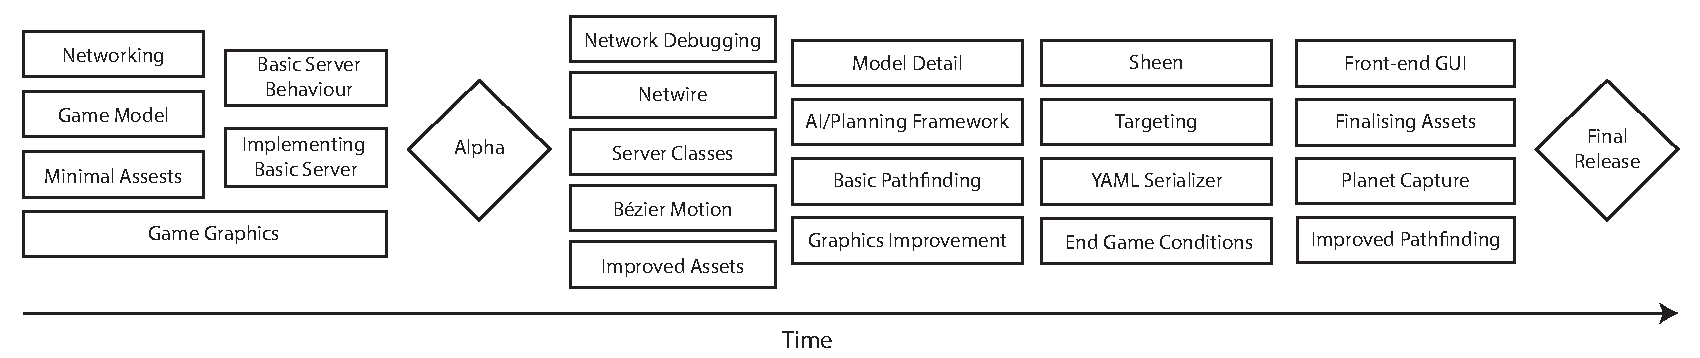
\includegraphics[height=33em]{res/pm/actual_workflow_diagram}
	\label{fig:actual_workflow_diagram}
	\caption{Actual workflow of project}
\end{figure*}

Casual conversation was issue throughout the course of the project, very often a concise meeting deteriorated into off-topic conversation and cost the project valuable time, the informal atmosphere in the project group exasperated the problem since the management roles couldn't failed as a part-time occupation, and there was no ``bad guy'' to keep the group focused on project work all the time.

Not only was it difficult to maintain a good working pace, but it became difficult to assess the appropriate amount of time to ask of each team member since the number of university contact hours per week fluctuated as modules began/ended and as other assignments were set.

\paragraph{Unavoidable issues}
One of the earliest issues arising with the schedule was attempting to arrange collaboration sessions which didn't conflict with any group member's other arrangements (particularly university assignments and contact hours). Rather than working asynchronously, the group decided to meet later in the evening and on weekends, when group members were tired and less productive, this meant the working hours became less and less productive, making milestones harder to reach on schedule as the project progressed.

An unavoidable issue in most projects is what's known as student syndrome, where people only start to fully apply themselves to a task in the last possible moment before a deadline.
%% CITE PROJECT MANAGEMENT BOOK
Although lack of motivation was never a problem, it was often the case that the team spent too much time perfecting something that is already of an acceptable quality, when there are other project components which desperately need work.

The most severe problem was having a slight underestimate of the time required for each project component. It's very difficult to accurately gauge how much work will be required to complete a particular task, and the schedule is almost always an underestimate. Even under the most efficient working conditions, the project gradually slipped further and further behind schedule until many unfinished components were under threat of being unfinished by the delivery date.

\paragraph{Conclusions drawn from time tanagement}
The initial scheduling of the project was overambitious, and it took quite a few emergency work sessions to bring the project back on schedule. Time could have been managed more effectively if the estimates were more realistic, however, an overestimate of time might have made the project team more prone to the aforementioned student syndrome, lower efficiency. Time estimation can is a double edged sword, since it takes a delicate balance to not damage the progress of the project by underestimating or overestimating, but in practice it's impossible to accurately predict how much time a certain tasks will take since the time required for debugging varies massively between bugs. 

The problem with scheduling in software projects is that any time allocated for fixing unknown bugs and fine tuning features can be used as a means for a developer to defer fixing detected bugs because they can be dealt with later, the problem being is that deferred bugs will then cost the project even more time because important issues weren't dealt with at the time, so not only will there be a context switching overhead for any deferred bugs, there may be extremely serious, yet undetected bugs that then cost the developers debugging time which hasn't been accounted for in the project schedule. One possible solution to such delays is to keep the entire team motivated to meet soft deadlines throughout the project so the team is kept forced to deal with delays promptly, that way the effect of delays for the overall project is largely mitigated. 
%tcq res 
% http://www.leonelson.com/wp-content/uploads/2005/04/projecttriangle.gif


\section{Development Model}
\label{sec:devmodel}

An agile approach to software development was chosen for this project. This methodology was
chosen because of its focus on rapid development and handling change. When working in a small
team, a heavy weight plan-driven development approach can dominate the actual process of development
due to the overhead. Sommerville states that using such an approach means that ``more time is
spent on how the system should be developed than on program development and testing.''\citepage{sommerville2011}{page 58}
In contrast, an agile approach is designed to deliver working software quickly so that changes
can be suggested and implemented in future iterations.

The agile method that was used was that of extreme programming developed by Kent Beck.\cite{beck1999}\cite{beck2000}
Extreme programming is an `extreme' approach to iterative development. Small releases are made
as quickly as possible. These releases are then evaluated and iterated on until a final release
that meets all requirements is delivered. Instead of planning and designing for the far future,
extreme programming advocates doing both of these activities --- bits and pieces at a time ---
throughout the entire project development lifecycle.

% Bad at frequent, formal release cycle

One core practice at the centre of extreme programming is testing and test driven development.
Test driven development, as described previously in section~\ref{sec:testing}, involves
developing test cases before coding the actual implementation. The benefits of test driven
development are a system that is thoroughly tested, reduced ambiguities in specification before
implementation begins, and avoidance of `test-lag'. However, Sommerville notes a few problems
that can be encountered when using test driven development:

\begin{enumerate}
\item Programmers prefer programming to testing. It is very tempting for a programmer to write
      incomplete tests, or skip test writing altogether, before moving onto the more rewarding
      task of implementation.

\item In some cases tests can be difficult to write. For example, testing user interfaces and
      display logic.

\item It is hard to judge the completeness of a test suite. There may be a large number of tests,
      but do they actually cover all of the code and all possible program execution.
\end{enumerate}

Although the Serenity project does include a test suite the team failed to stick to the test
driven development tenet of extreme programming. This was mainly caused by the first issue
pointed out by Sommerville. The team preferred to go straight into implementing a feature or
enhancement and then, maybe, write tests after the fact.

Another important practice in extreme programming is that of pair programming. Two developers
work in tandem at the same computer. One programmer, the driver, actively writes the implementation
of the program. The other, the observer, continously reviews each line of code as it is typed 
and thinks about the direction of the work.\cite{williams2001} There are a couple of major advantages
to pair programming:

\begin{enumerate}
\item It is an informal code review process that can be very effective at discovering errors
      as the code is written.

\item It promotes collective ownership and responsibility for the component being worked on.
      Code is not `owned' by an individual who may dislike others working in the same area or
      be demotivated by critism during code reviews, similarly one individual is not held responsible
      for any problems.
\end{enumerate}

Studies have shown that pair programming may have little effect on overall productivity, but
creates a substantial reduction in errors in the code.\cite{cockburn2000} This is prescribed
to the continuous code review that occurs, and a decrease in false starts and redoing work.

Pair programming was an effective technique that was used throughout the development of
Serenity. The experience lead to the conclusion that pair programming is a good method for
development for the advantages mentioned above as well as the following reasons:

\begin{description}
\item[Problem solving] When a problem is encountered two people are able to discuss it together
which often helps either or both of them coming up with a solution quicker than they would
individually.

\item[Learning] Knowledge is constantly exchanged within the pair. So after a component
has finished and the pair move on to other work they have both become more effective programmers
in some way.

\item[Team building] Working together lead to better communication and enhanced teamwork.
This made the project team a more effective work group.
\end{description}

However, due to such a small team it was felt that it would be impossible to work on all
tasks in pairs and still finish the work within the time constraints. Therefore, some work
was done individually, but still always trying to work in close proximity to enable teamwork
where necessary.

\section{Project Control}
\label{section:control}

% Control Measures examined and critiqued
% ie change requests

Lorum ipsum sit dolor amet.\citefix{church1932}  \lipsum[2-4]

\section{Stakeholders and Communication Plan}
\label{section:communication}

The various parties identified as stakeholders are shown in Table \ref{tab:stakeholders} (overleaf). The relationship between the stakeholder and the project is shown, along with a rough estimate of their power and interest.\sidenote[][-2em]{See \bibentry{mendelow1991stakeholder}} This grid will form a reference for making sure that all interested parties are communicated with appropriately throughout the duration of the project.

\noindent Communication within the project team is examined in detail elsewhere in this document, so the remainder of this section is concerned with the other stakeholders.

\vspace{1em}

\begin{table*}
	\footnotesize
	\renewcommand{\arraystretch}{1.5}
	\begin{tabular}{p{9em} p{5em} p{3em} p{3em} p{9em} p{9em} p{9em}}
		\toprule
		\emph{Stakeholder} & \emph{Relationship} & \emph{Power} & \emph{Interest} & \emph{Requirements} & \emph{Measurements} & \emph{Communication Strategy} \\
		\midrule
		
		Project Team & Internal & High & High & 
		Good working environment, creative input. & 
		Meeting project spec, good grades! & 
		Various, detailed elsewhere. \\
		
		Supervisor --- Sara Kalvala & Internal & High & High & 
		Good communication. & 
		Adherence to spec, good PM, high quality write-up. & 
		Weekly meetings. \\
		
		Client --- Matt Leeke & Core \mbox{External} & High & High & 
		Good communication, creative input, hard work & 
		Strength of software, strength of report & 
		Weekly meetings. \\
		
		Second Assessor & Core \mbox{External} & High & Low & 
		None & 
		Marking scheme & 
		Deliverables only. \\
		
		Projects Organiser --- Steve Matthews & External & High & Low & 
		Cooperation when required. & 
		Deliverables on time. & 
		Email or meeting if required. \\
		
		Playtesters & External & Low & High & 
		Able to report issues / feature requests. & 
		Strength of game, input considered. & 
		Email. \\
		
		Other future users & Rest of World & Low & High & 
		Game works and is reliable. & 
		Strength of game, re-playability. & 
		Website, forums, blog. \\
		
		The Haskell and FP Communities & Rest of World & Low & High & 
		None & 
		Interest in  / strength of results and tools released. & 
		Online as above, and via the final report. \\
		\bottomrule
	\end{tabular}
	\vspace{1.5em}
	\caption[][1em]{Stakeholders for the project.}
	\label{tab:stakeholders}
\end{table*}

\subsection{Supervisor Meetings}

Regular communication with the project supervisor is likely to be a critical factor in success of the project. For this reason a weekly meeting with at least one member of the group if not more will be high priority.

\subsection{Client Meetings}

The client is clearly vital to the success of the project, and continual feedback on each release will allow for early identification of any problems. At least one meeting per release (ie each week) will be required, as well as further meetings and correspondence as needed.

\subsection{Projects Organiser and Second Assessor}

The projects organiser could exert a strong influence over the project if they wished, but as there are many projects and it would be inappropriate for them to demonstrate partiality, extended levels of communication are unlikely to be necessary. Brief updates pertaining to deliverables is all that should be required. But if the project organiser initiates communication then they should be made a high priority.

Communication with the second accessor is, for the most part, not appropriate, excepting when within the remit of the deliverables, i.e. the report and presentation themselves.

\subsection{Playtesters and End Users}

End users are clearly important to the goals of the project, but they will have little interest or influence in the early stages. Online updates, an email to report bugs to, and a mailing list for any events that are organised will be sufficient communication.

\subsection{The Haskell and Functional Programming Communities}

The overall end goal of the project is not just a game, but an examination of Haskell and Functional Programming as a game development environment. However the Haskell community at large is unlikely to have much interest in the project while it is running. Communication back to the community should therefore be largely via the final report, as well as the methods for end users above.



\section{Team Structure}

% Team Structure, management and leadership

Lorum ipsum sit dolor amet.\citefix{church1932}  \lipsum[2-4]
\section{Risk Management}



Lorum ipsum sit dolor amet.\citefix{church1932}  \lipsum[2-4]
\section{Evaluation of Tools and Techniques}
\label{sec:tools}

A number of different tools were used in the day to day running of the project.
These tools were used to ease the collaboration between members by ensuring that everyone knew
what they were supposed to be doing and how to share it with the others.

\subsection{Source Control: Git}

Source control systems are an essential tool for software projects, especially those
with multiple developers. Using source control to easily track the changes to source
code is helpful because, as McConnell explains, having a history of changes helps a
developer to identify the origin of bugs quickly.\citepage{mcconnell2004}{page 667}

The Git source control system\sidenote{\url{http://git-scm.com/}} was chosen for this project.
Git was chosen for a number of reasons. Firstly, it has a lightweight branching model which
allows for quick creation of new development branches for experimental features independent of
any other development. Chacon notes this as Git's ``killer feature''.\citepage{chacon2009}{page 38}
Another reason for choosing Git is its distributed nature. Every user has a full clone of the
entire repository that can act as a replacement for any other instance of the repository; this means
that there is no single, centralised point of failure.

A centralised master repository was hosted on Github, a popular code host.\sidenote{\url{https://github.com/}}
This made it easier for team members to share their changes to the code base. Once a change has been made
it can be `pushed' to the Github repository; other team members can then `pull' it to their local
repositories.

Git was an ideal source control system for the project. Not only does it allow the users to see
the entire history of changes made to the project it makes collaborative development between
multiple team members incredibly easy. Instead of having to resolve conflicting changes to files
it is possible to use the built in merge tool to combine the work of two or more people on the
same set of files with minimal effort. Git is recommended for all future development projects.

\subsection{Tracking and Managing Releases: Trello}

\begin{marginfigure}
	\includegraphics[width=6cm]{res/trello.png}
	\caption[Trello]{Project Serenity's Trello page}
	\label{fig:trello}
\end{marginfigure}

Trello is a modern, online take of an age old concept --- a wall of post-its. Trello allows for overall planning of tasks and communication between members in a highly dynamic, fluid way. Cards are arranged into a list-of lists, each list being some kind of functional decomposition or `stovepipe'. Trello has been used in the project to track the requirements for each weeks releases, but still allowing rapid changes to be made and communicated.

Trello acted as a useful reference to the current state of the project: what tasks are planned and who is doing them.
It is a good tool for keeping a small group of people organised, but requires careful management to keep it
up to date and useful.

\subsection{Bug Tracking: Github Issues}

Trello does not entirely alleviate the need for a full bug tracker. When working of development of
individual features and components it was necessary to have a method of tracking more transient issues
and tasks. The initial plan was to use the service provided by Fogbugz, a stand alone bug tracking
web application. However, in the end the Issues feature built into Github hosted repositories was
used. This was decided because it reduced the number of third party services that were relied upon
and it provided better integration with the hosted repository itself. Although it is much more minimal
than Fogbuz, it provided enough features, such as milestones, labels, email notifications, and
issue assignment, for this project.

An issue tracker was very useful for noting down smaller tasks and bugs that cannot be fixed immediately,
but must not be accidentally forgotten about. If a project is using Github to host code then the
Issues component is recommended if only simple issue tracking features are required. However, for
more complex requirements a more fully featured service may be a better option.

\subsection{Backups}

Backups of the source code and other project assets are essential. In the event of a
disaster, such as losing a computer to a fire, it must be possible to recreate the
entire project in its latest state quickly and without any repetition of work.\citepage{mcconnell2004}{page 669}
The use of Git and Github for source control made it simple to ensure that all
source code was located on multiple computers. By `pushing' commits to the Github
repository all code was stored in the cloud. When other team members `pulled' the code
later on it was then mirrored on their computers as well. Extra precautions were taken
by also `pushing' the Git repository to private servers owned by the team members.
Also, the free service provided by Dropbox\sidenote{\url{https://www.dropbox.com/}}
was used to share and backup any other files, such as assets and planning notes.

Fortunately a situation which required recovery from backups was never encountered,
but the strategies put it place should have been more than adequate if the need ever
arises in the future. Since the main backup strategy was part of normal development
workflow it was impossible to forget to implement it. However, it does have to be ensured that
all members are sharing their changes as frequently as possible (even if a feature is
not fully finished) to prevent any work in progress from being lost in case an individual's
computer dies. The extension to this core backup strategy, storing the repositories
on other personal servers, was easy because of Git's feature set which was designed
to be distributed in nature and so allows tracking and updating of multiple remote repositories.

\subsection{Continuous Integration: Jenkins}

Section~\ref{sec:testing} introduced the idea of continuous integration as a method
of regularly running the test suite and performing a full build of the software.
The Jenkins continuous integration server\sidenote{\url{http://jenkins-ci.org/}}
was used for this project. Jenkins was chosen because it is a widely used open
source project.\sidenote{\url{http://stats.jenkins-ci.org/jenkins-stats/}}
Jenkins also works well with projects hosted on Github because of its Github plugin\sidenote{\url{https://wiki.jenkins-ci.org/display/JENKINS/GitHub+Plugin}}
and Github's Jenkins specific post-receive hook.

Although Jenkins does not have a very good user interface it suited the needs of
this project. It was a good tool for running a test suite with every change to the
code base and ensuring that the game would build correctly. Email notifications on failure
were useful, but also relatively noisy at times. Continuous integration is probably
more useful for more mature projects that need to ensure that changes do not introduce
any regressions than it is for a project in the early stages of development when a lot
of features are not fully working.

\chapter[Requirements]{Requirements}
\label{ch:requirements}

\chapterepigraph{``All things are created twice; first mentally; then physically.  The key to creativity is to begin with the end in mind, with a vision and a blue print of the desired result."}{ Stephen Covey}

\newthought{Starting a sentence} with a new thought.


% help site at http://www.projectmanagementhelp.com/how-to-write-functional-requirements/
% bullet point these requirements, describe them, specify any details.
% include bain quite as footnote
\section{Functional Requirements}

% what it is 
% what it will be used for
% how we will measure success

\begin{enumerate}

\item AI:
The AI, artificial Intelligence will include any algorithms under the field of Artificial Intelligence, such as planning.
The Player's fleet will be controlled by an AI algorim. It will use a planning algorithm that takes a high level objective given by the player, and generates a series of steps to achieve that objective.
The measurement of success for AI is being able to give an order to a ship that requires at least 3 sub steps to achieve that goal, and the AI successfully completing that goal(assuming it is possible to achieve this goal).
When an AI is given a goal that is either impossible to achieve given the world state, or is later invalidated due to world changing before the goal is achieved, the goal will be canceled, and the AI will wait for the next goal assigned by the player.

\item Realtime Strategy:


\item Multiplayer:
Multiplayer is a game which two human players can participate in, interacting with each other within the game world.
For this specific game, both players will be operating different computers on the same Network.
The network requirements are that it is a Local Area Network, allowing much greating bandwidths than the World Wide Web.

\item Ship Design:


\item Resource System:

\item Planetary Capture:

\item Campaign Style Multiplayer:

\item Tactical Zoom:

\item Fog Of War:

\item Operating System Requirements:
Mac OS or Linux(kernel 2.6 or later) 

\item Haskell:

\end{enumerate}


\section{Non-Functional Requirements}




functional - 2d, realtime strategy, multiplayer, ship design, resource system, ai, planetary capture resource system, possiblity of campaign style multiplayer, tactical zoom/gameplay, fow, hw requirements, haskell.
non-functional - fun, reliable, secure, short lived game sessions, 

\section{Conclusions}

% Assessment of our key decisions
% Conclusions on Haskell

Lorum ipsum sit dolor amet.\citefix{church1932}  \lipsum[2-4]

\chapter[Summary of Conclusions]{Summary of Conclusions}
\label{ch:conclusions}
%\containsfigures{Summary of Conclusions}
%\containslistings{Summary of Conclusions}
%\containstables{Summary of Conclusions}

\chapterepigraph{Haskell is an abstract research language used only in academia, education, banking, stock trading, circuit design, embedded systems, cryptography, operating systems research, bioinformatics, phone apps, and web services.}{Jafet, quoted in \emph{Haskell Weekly News} Issue 265}

\newthought{Brief intro} for this section. \lipsum[4]

\lipsum[4]

\appendix
\chapter[--- Monads and Other Fundamental Haskell Design Patterns]{--- Monads and Other Fundamental Haskell Design Patterns}
\label{app:monads}
%\containsfigures{Monads and Other Fundamental Haskell Design Patterns}
%\containslistings{Monads and Other Fundamental Haskell Design Patterns}
%\containstables{Monads and Other Fundamental Haskell Design Patterns}

\emph{This section could be dropped if there is no time to write it, and replaced by references to online tutorials.}

\section{Functors}

\section{Applicative Functors}

\section{Monads}

\section{Monad Transformers}

\section{Monoids}

\section{Category Theory}

\backmatter
\chapter{Acknowledgements}

\begin{fullwidth}

\lipsum[1]

\vspace{1em}\noindent
This report makes extensive use of the Tufte Latex class written by Bil Kleb, Bill Wood, and Kevin Godby (\url{http://code.google.com/p/tufte-latex/}). 
The Haskell code in this report was typeset using a modified version of Lambda\TeX\ originally created by Patryk Zadarnowski (\url{http://www.jantar.org/lambdatex/}).

\end{fullwidth}

\begin{fullwidth}

\def\bibname{Full Reference List and Selected Bibliography}
\nocite{*}
\bibliographystyle{plainnat}
\addcontentsline{toc}{chapter}{\bibname}
\bibliography{references}

\end{fullwidth}
\printindex

\end{document}

